\chapter{Other low-energy physics with P-type point contact detectors}

In this section, we basically discuss two things: Heavy non-relativistic axions, the signal, and the exclusion limit as calculated with the data from the previous chapter.

Also, making some reasonable assumptions about Majorana, we make some estimates as to the sensitivity of the Majorana experiment to WIMP dark matter and axion dark matter (via the axioelectric effect).  

		
	\section{Other dark matter: heavy axions}
	\label{sec:CalcLimitsOnHeavyAxions}		
		


	\subsection{Heavy axion signal}
	\label{sec:CalcLimitsOnHeavyAxionSignal}		

	The signal for a non-relativistic axion interacting via the axioelectric effect has been derived in~\cite{Pospelov:2008jk}.  This particular inelastic interaction involves the deposition of the \emph{complete} energy of the axion which, in the non-relativistic case, is essentially equal to the mass of the particle.  Since the excitation of the electron via the axioelectric effect is similar to that mediated by a photon in the photoelectric effect, the signal is a delta function centered at the mass of the axion, $m_{a}$.  Convolved with the detector resolution, the signal would appear gaussian with width exactly that of a gamma or x-ray of energy equivalent to $m_{a}$.  The rate of this interaction has been estimated in~\cite{Pospelov:2008jk} as:
	
		\begin{equation}
			R \left[ kg^{-1} day^{-1} \right]\simeq \frac{1.2\times 10^{19}}{A} \gaa^{2} m_a \sigma_{photo}
			\label{eqn:AxioelectricRate}
		\end{equation}

where $A$ is the atomic mass, $m_{a}$ is the mass of the axion in keV, $\sigma_{photo}$ is the measured photoelectric cross section in barns, and $g_{a\bar{e}e}$ is the dimensionless coupling constant.  In the derivation of this result, the value of the density of the dark matter $\rho_{D}$ = 0.3~GeV cm$^{-3}$ was used.  The rate calculated for a germanium detector ($A=72.96$) with a chosen coupling constant, $\gaa = 10^{-11}$, is given in Figure~\ref{fig:HeavyAxionSignalRate}.  The rate calculation used well-known cross sections obtained from the NIST FFAST database located online~\cite{chantler:597}.  

The low noise of PPC detectors yields excellent sensitivity to non-relativistic axions with masses $\leq10$~keV due their sharp resolution at low energies.  A comparison of an axioelectric signal at a given $\gaa$ is provided in Figure~\ref{fig:ResCompare} for characteristic resolutions of NaI and germanium detectors.  In this plot, it is clear that the improved resolution of the germanium detector allows less smearing of the signal, forcing more counts into a narrower peak.

		\begin{figure}
			\centering
			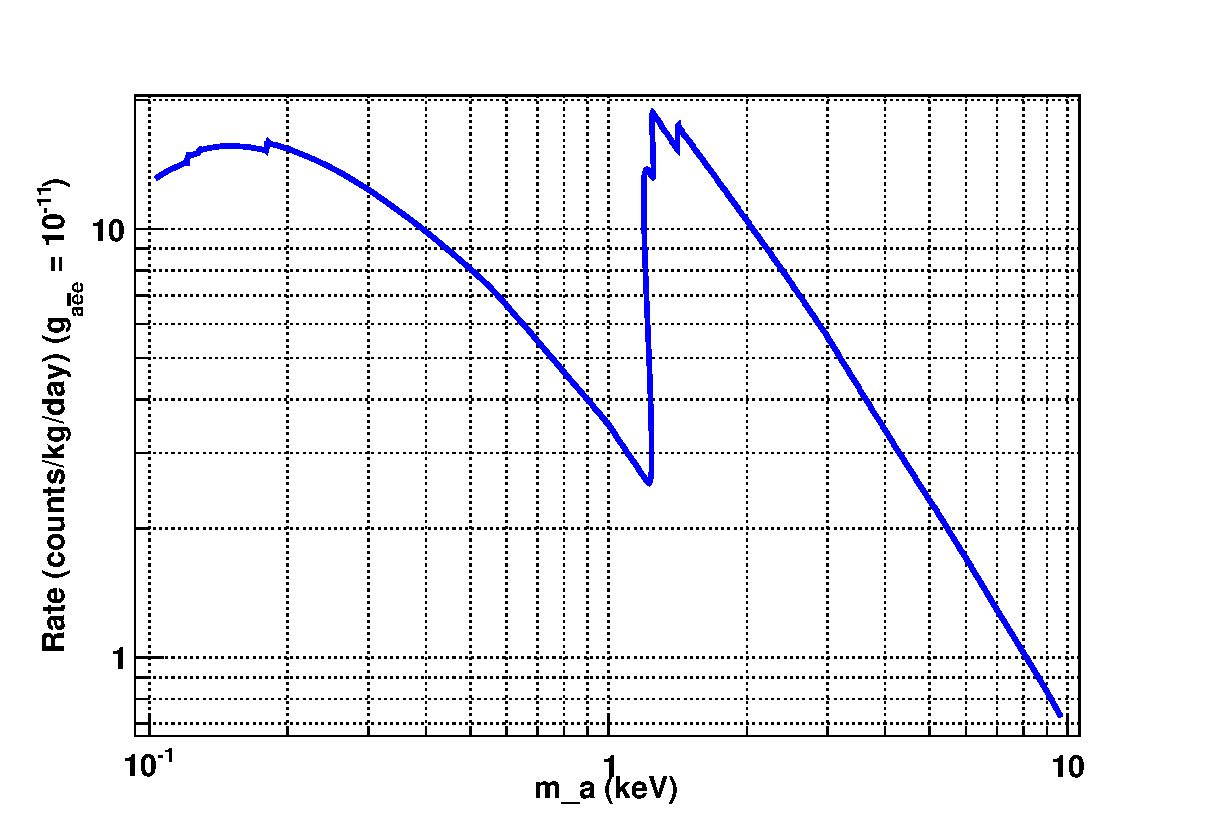
\includegraphics[width=0.9\textwidth]{GeRate}
			\caption[Axioelectric interaction rate in germanium]{Non-relativistic axion axioelectric 
			interaction rate in germanium.  The photoelectric cross section for germanium was obtain
			from the NIST database~\cite{chantler:597}.}
			\label{fig:HeavyAxionSignalRate}
		\end{figure}

		\begin{figure}
			\centering
			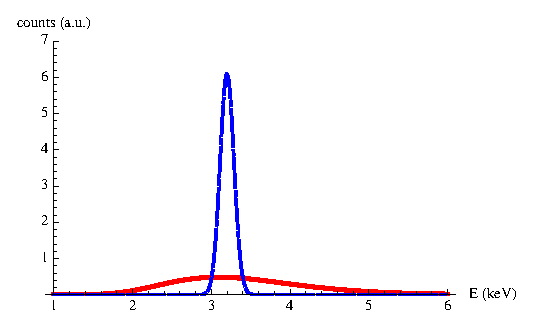
\includegraphics[width=0.9\textwidth]{DAMARes}
			\caption[Axion signal at $m_{a}$ = 3.2~keV]{Axion signal at $m_{a}$ = 3.2~keV comparing 
			the detector responses of germanium (blue, dashed) and NaI (red, solid) to an equivalent
			$\gaa$.  }
			\label{fig:ResCompare}
		\end{figure}

	\subsection{Limits on the axioelectric effect}
	\label{sec:CalcLimitsOnHeavyAxionLimits}		
		
	Limits were calculated using the profile-likelihood method described in Section~\ref{sec:LimitsML}.  Fit were performed on the complete number of data sets described in Chapter~\ref{chap:AnalysisBeGe}, with a total livetime of 150.6~days.  All data sets yielded similar results and so one data set was chosen with 95\% rise-time acceptance cuts and microphonics cuts applied.  As outlined before, assumptions about the source of slow-rise-time events reduced the fidudical mass to 0.33~kg (see Section~\ref{sec:BeGeLowEnergyFeatures}).  Additionally, results with unbinned and binned maximum-likelihood fits were consistent and so the former was used.  The limit calculation followed the same procedure as a peak search in the data and is outlined as follows:
		\begin{itemize}
			\item Define the gaussian signal $f_{axion}$: 
			\begin{itemize}
				\item Choose mass $m_{a}$ of the axion defining $\mu$ of gaussian
				\item Determine $\sigma$ at $E = m_{a}$ using resolution in Equation~\ref{eqn:SigmaEqn}.
			\end{itemize}
			\item Fit to the function $B + N_{axion} f_{axion}$ where $B$ is the background defined in Section~\ref{sec:LimitsDataAndModel} and determine the profile likelihood $\plln$.
			\item Determine the 90\% upper limit on $N_{axion}$ using $\plln$.
			\item Repeat for other values of $m_{a}$
		\end{itemize}		
	
	During the fits, the $\mu$ and $\sigma$ of the gaussian signal, $f_{axion}$, were kept fixed and only the amplitude, $N_{axion}$ was kept as a free parameter of the signal.  For the background, the behavior of the parameters was the same as during WIMP exclusion fits (see Section~\ref{sec:LimitsDataAndModel}) and the relative amplitude of the \gersixeight~and\znsixfive~L-lines was kept fixed as described in Section~\ref{sec:LimitsConstrained}.  Fixing this relative amplitude served to minimize the impact of the L-lines in the exclusion fits since a signal centered at 1.1 and 1.3~keV would look exactly like the L-capture lines.  The difficulties seen while determining limits on low-mass WIMPs did not appear in these calculations because the signal (gaussian centered at $m_{a}$) was not similar to the background except for the case of the L-lines.  The value of the axion mass was scanned from 0.1~keV to 7.8~keV in steps of 0.2~keV using both high- and low-gain channels: high-gain channel, $0.1\to2.9$~keV; low-gain channel, $3\to7.8$~keV.  The axion mass was allowed to vary below threshold (0.5~keV) because the finite resolution of the detector would allow portions of the expected gaussian signal to be detected above threshold.  An example of an exclusion fit in the high-gain channel is shown in Figure~\ref{fig:ExampleHeavyAxionFit} for $m_{a}=3$~keV.  

		\begin{figure}
			\centering
			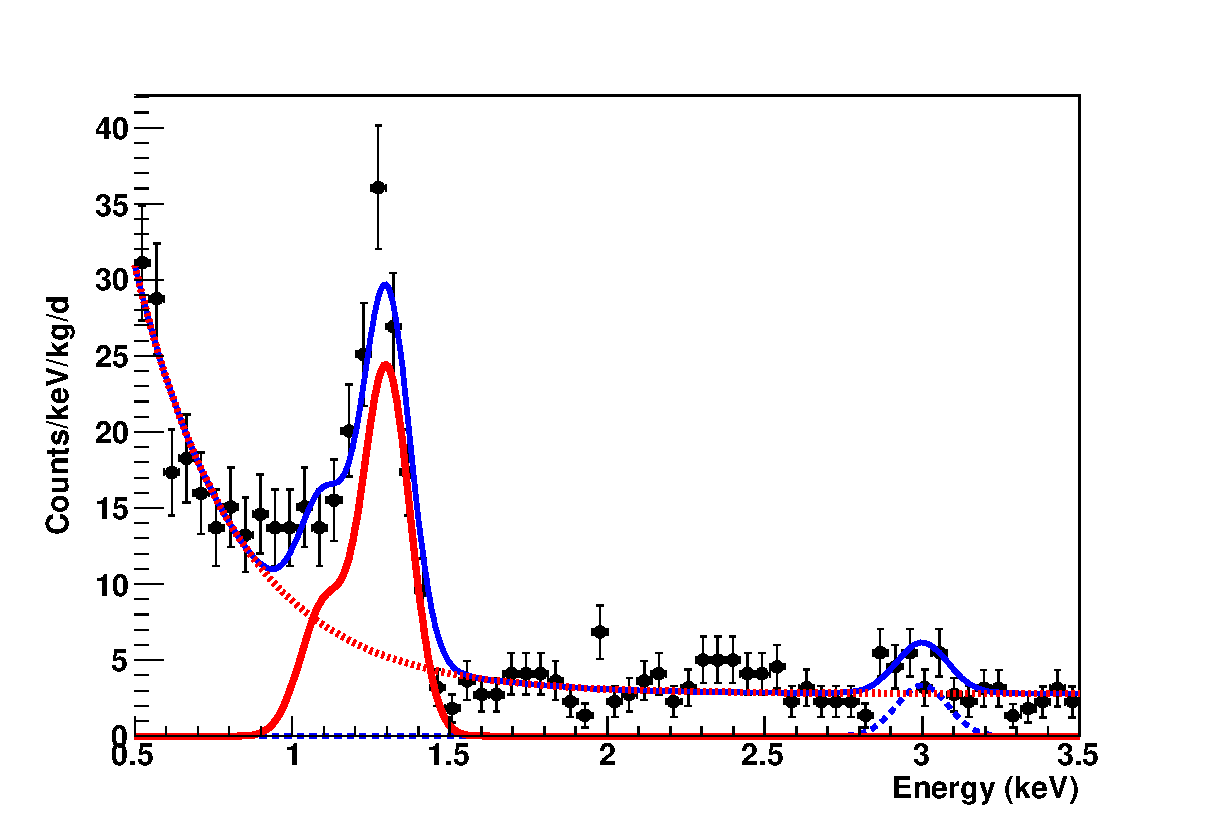
\includegraphics[width=0.9\textwidth]{AxioelectricFitExample}
			\caption[Example of an excluded non-relativistic axioelectric signal at $m_{a}=3$~keV at 
			90\% CL]{Example of an excluded non-relativistic axioelectric signal at $m_{a}=3$~keV at 
			90\% CL.  In this fit performed in the high-gain channel, the excluded value $N_{axion}$ 
			is 36.1 counts.  
			The components of the fits are split: red solid, L-Lines; red dotted, flat plus exponential
			background; blue dashed, excluded axioelectric signal.}
			\label{fig:ExampleHeavyAxionFit}
		\end{figure}
			
	The 90\% CL excluded rate in counts/kg/day, $R_{axion}(m_{a})$, was determined from $N_{axion}(m_{a})$ and from this value the upper limit of $\gaa$ could be determined.  The exclusion calculated from this result is presented in Figure~\ref{fig:HeavyAxionLimits} along with a comparison to other results, including previous results of the CoGeNT collaboration~\cite{Aalseth:2008aa}, the CDMS collaboration~\cite{Ahmed2009}, and an acceptance region from the DAMA collaboration~\cite{Bernabei:2005ca}.  As noted in both references~\cite{Collar:2009sp,Pospelov:2008jk}, the limit calculation performed in~\cite{Bernabei:2005ca} did not correctly treat the leading term in Hamiltonian producing instead a reduced rate for a given $\gaa$ around 3 orders of magnitude lower.  The corrected result from DAMA as outlined in~\cite{Collar:2009sp} appears in Figure~\ref{fig:HeavyAxionLimits}.
			
		\begin{figure}
			\centering
			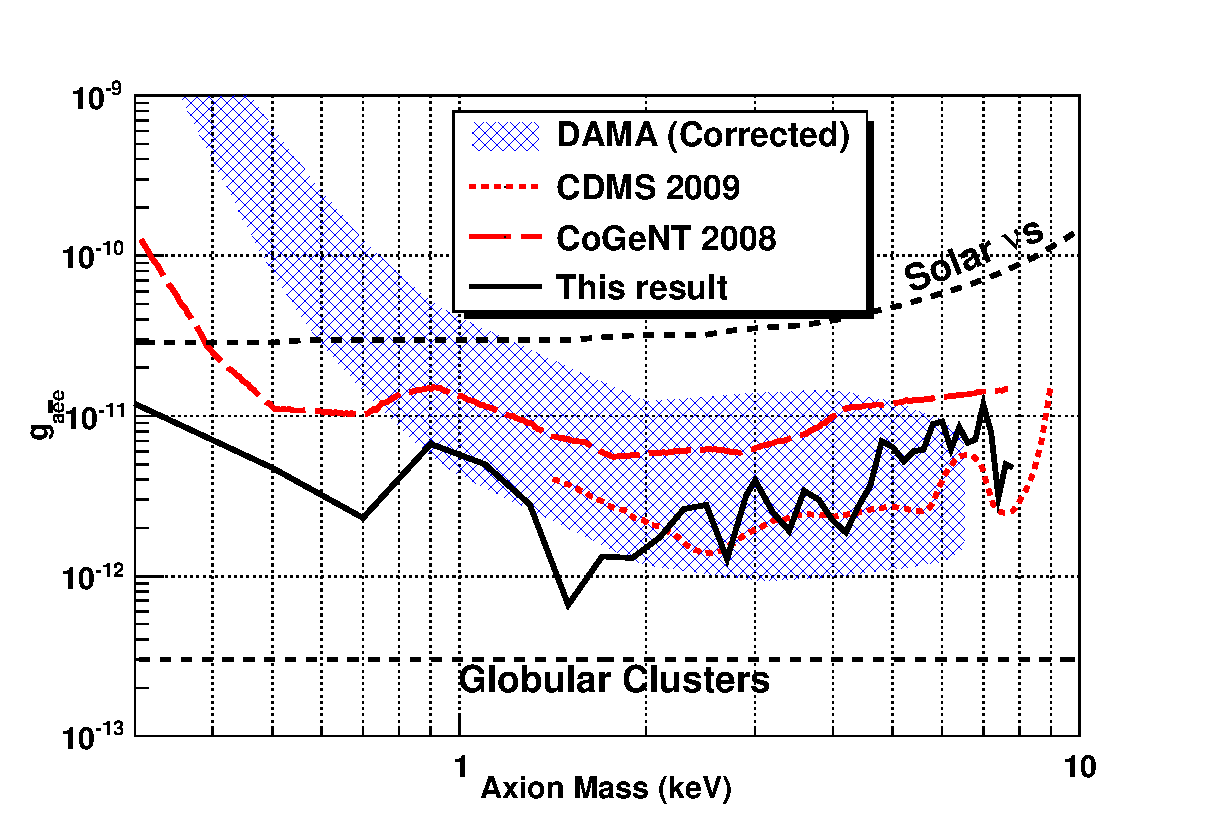
\includegraphics[width=0.9\textwidth]{axion_constrained_unbinnedall_exclusion_plots_final}
			\caption[Limits on the axioelectric coupling constant $\gaa$]{Limits on the axioelectric 
			coupling constant $\gaa$.  Results from this work appear in comparison to previous 
			results from CoGeNT~\cite{Aalseth:2008aa}, CDMS~\cite{Ahmed2009}, and 
			DAMA~\cite{Bernabei:2005ca}.  The DAMA results have been corrected per 
			reference~\cite{Collar:2009sp}.}
			\label{fig:HeavyAxionLimits}
		\end{figure}
		
	\subsection{Conclusions and Discussion}
	\label{sec:DiscOnHeavyAxionLimits}	


							
	\section{Sensitivity of the \MJ~\minmod~to a Dark Matter signal}
	\label{sec:MJSensitivity}
	
	Since a framework was established to determine exclusion limits for low-mass WIMPs and for the axioelectric coupling constant, it is simple to apply this to determine the sensitivities of the \MJ~\minmod.  Calculating the sensitivity of the experiment involves making some assumptions of the background at low energies and of the structure of the experiment.  A discussion about the estimation of the background is given in the following in Section~\ref{sec:MJLowEnergyBackgroundModel}.  The general prescription for calculating the sensitivity is as follows:
	
		\begin{itemize}
			\item Generate a background model, including an expected rate of background
			\item Simulate a spectrum according to the background model
			\item Fit to the simulated spectrum the background model plus a signal model (e.g.~WIMP or axioelectric spectrum)
			\item Calculate the upper limit on the amplitude of the signal
			\item Repeat a large number of times to generate an ensemble of limits.
		\end{itemize}	
Details regarding this procedure will be outlined in the following.  Details of the \MJ~\minmod are given in Chapter~\ref{chap:Majorana}.  For these purposes, we have assumed that the \MJ~\minmod~is composed of 20~kg of material, though in reality it will likely have at least twice as much material added, and that it will run to accumulate between 1 and 5~years of livetime.  
	
		\subsection{Low-energy background model}
		\label{sec:MJLowEnergyBackgroundModel}
		
The estimation of background generally comes from verified simulations and from extrapolations from previous experiments.  In this work, the background is estimated by assuming it arises from two main sources: (1) a continuum from higher energy processes, and (2) counts from the beta decay of cosmogenically-produced tritium in the detector.  A simulation to estimate (1) is wrought with challenge since a large number of contributions can effect the result.  However, it is possible to use previous results from other germanium-based experiments to produce an estimate of this background.  The IGEX experiment measured a flat background rate of $\sim0.1$~counts/keV/kg/day in this low energy region ($4\to10$~keV)~\cite{Ira01}.    The \MJ~\minmod plans to reduce background above 200~keV by a factor of 100~\cite{MajoranaWhitePaper} and so it is reasonable to expect the flat background at low energies will follow this same reduction to be roughly 0.001~counts/keV/kg/day.  

The estimate of a background to tritium involves understanding the activation rate of tritium at the surface of the earth.  After 
		
		\subsection{WIMPs}
		\label{sec:MJSensitivityToWIMP}
		
			\begin{figure}
				\centering
				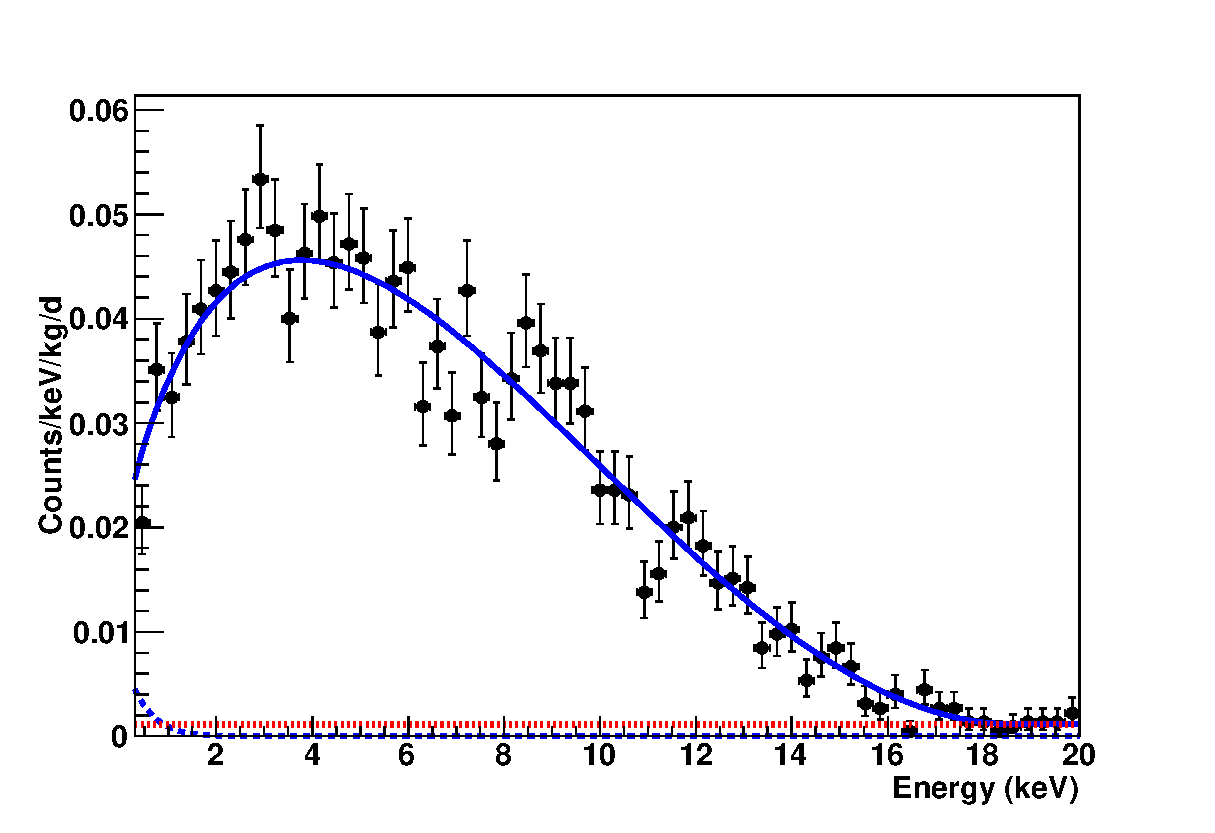
\includegraphics[width=0.9\textwidth]{MJDemoExampleSensFit}
				\caption[\MJ~\minmod WIMP sensitivity fit example.]{A sensitivity fit example with WIMP  
				signal at $M_{W}=10$~GeV, with $\signuc$ excluded at 90\% CL with value
				 $8.6\times10^{-9}$~pb.  Components of the fit are broken out including WIMP 
				 signal (blue dashed) and flat background (red dotted).  The major feature in the 
				 fit is due to the beta spectrum of tritium.}
				\label{fig:MJSensitivityToWIMPExample}
			\end{figure}
	
			\begin{figure}
				\centering
				\def\figheight{0.41\textheight}				
				\subfigure[1~year (20 kg-yr) exposure time]{
					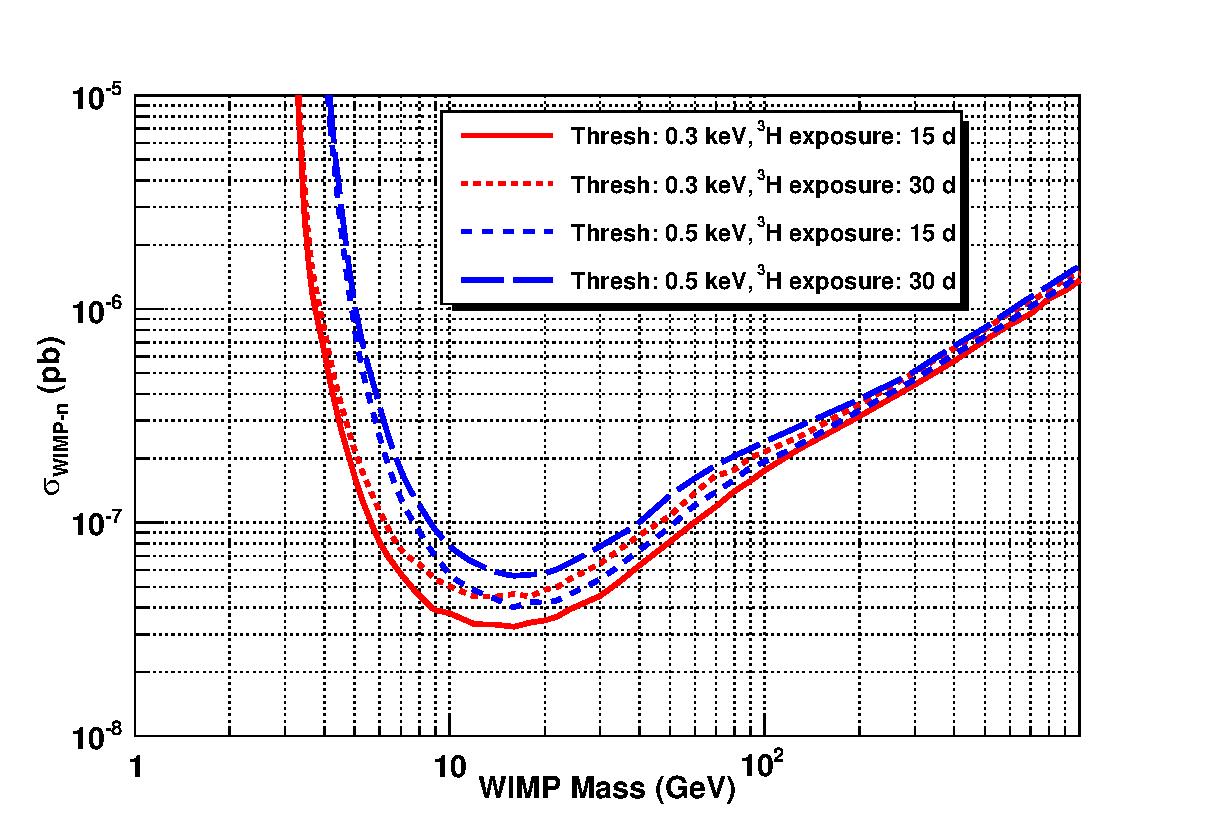
\includegraphics[height=\figheight]{20TimeExposureMJ}
					\label{fig:20TimeExposureMJ}						
				}
				\subfigure[5~year (100 kg-yr) exposure time]{
					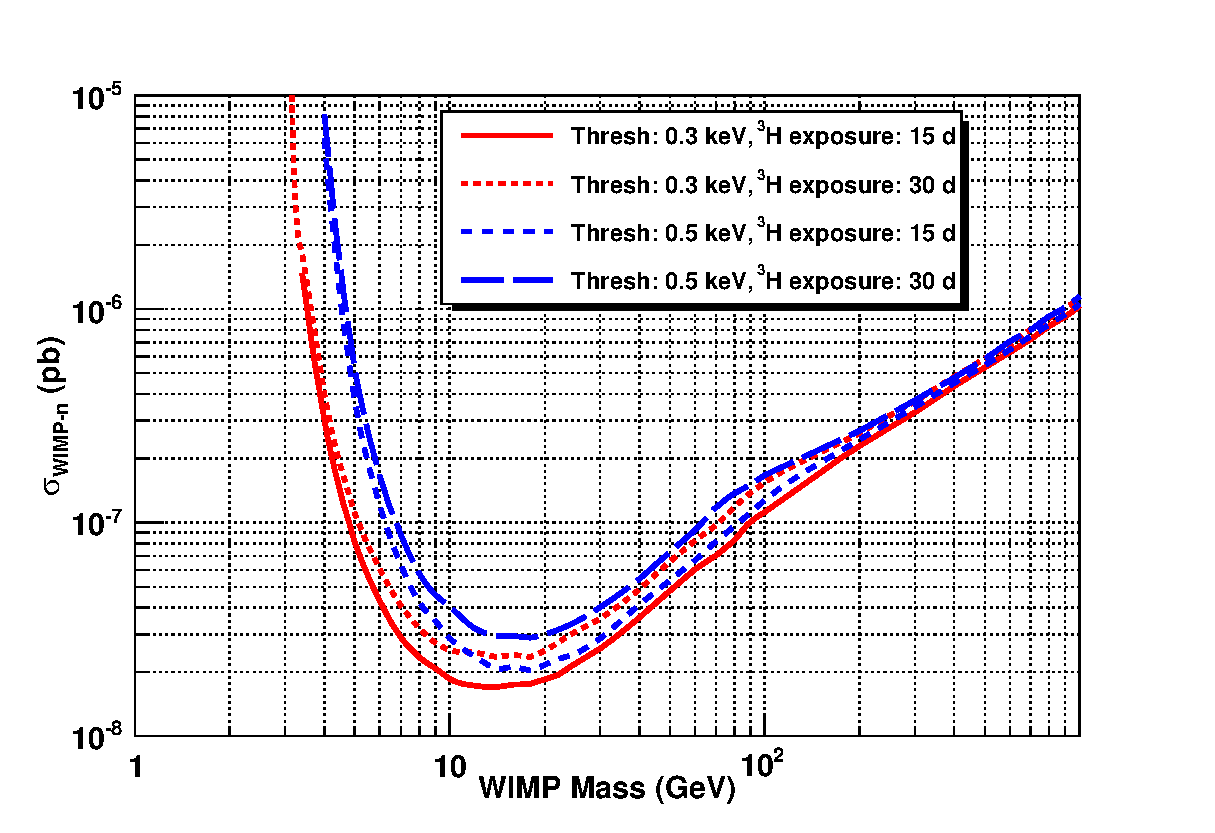
\includegraphics[height=\figheight]{100TimeExposureMJ}
					\label{fig:100TimeExposureMJ}						
				}				
				\caption[\MJ~\minmod~sensitivity to a WIMP signal]{\MJ~\minmod~sensitivity to a
				 WIMP signal.}
				\label{fig:MJSensitivityToWIMP}
			\end{figure}		
		
			\begin{figure}
				\centering
				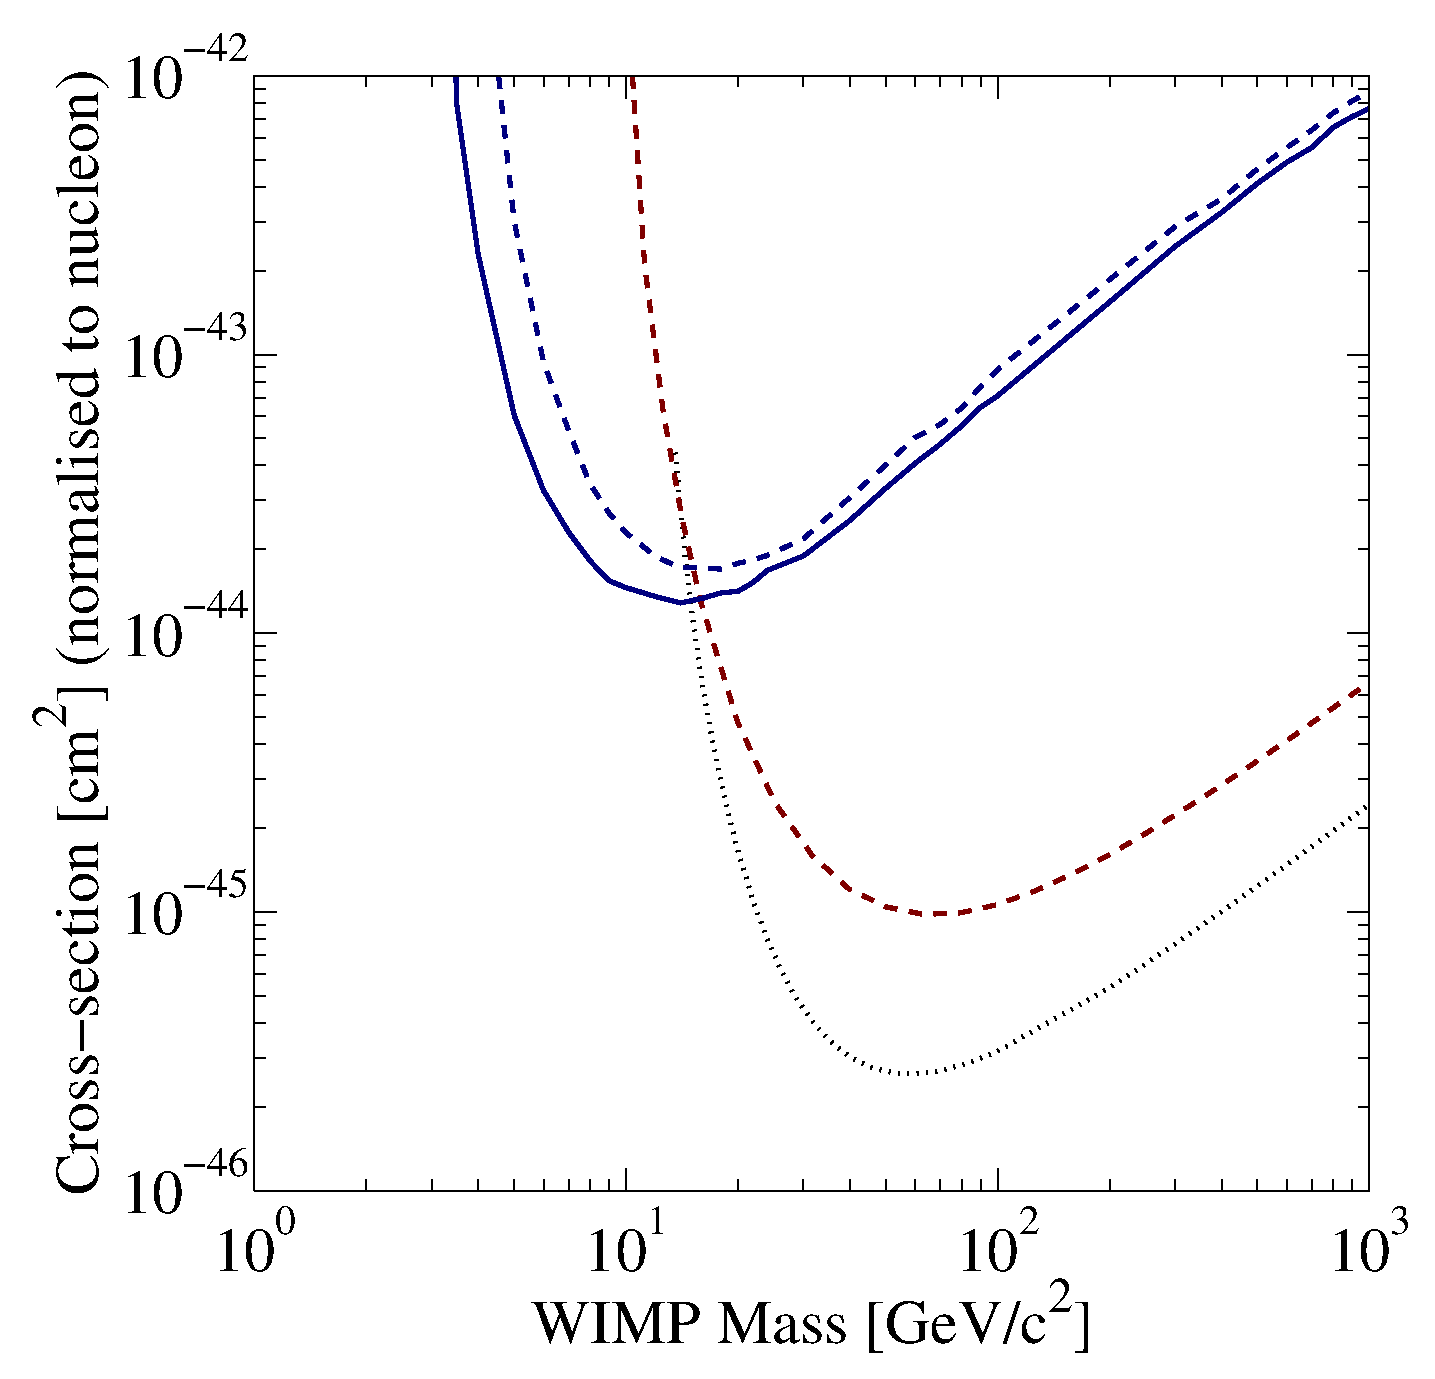
\includegraphics[width=0.9\textwidth]{MGM_MJ_Sensitivity_Compare}
				\caption[\MJ~\minmod~sensitivity to a WIMP signal, comparing to other experiments]
				{\MJ~\minmod~sensitivity to a WIMP signal, comparing to other experiments.}
				\label{fig:MJSensitivityToWIMPCompare}
			\end{figure}			
			
		\subsection{Heavy axions}
		\label{sec:MJSensitivityToAxions}
		
		
			\begin{figure}
				\centering
				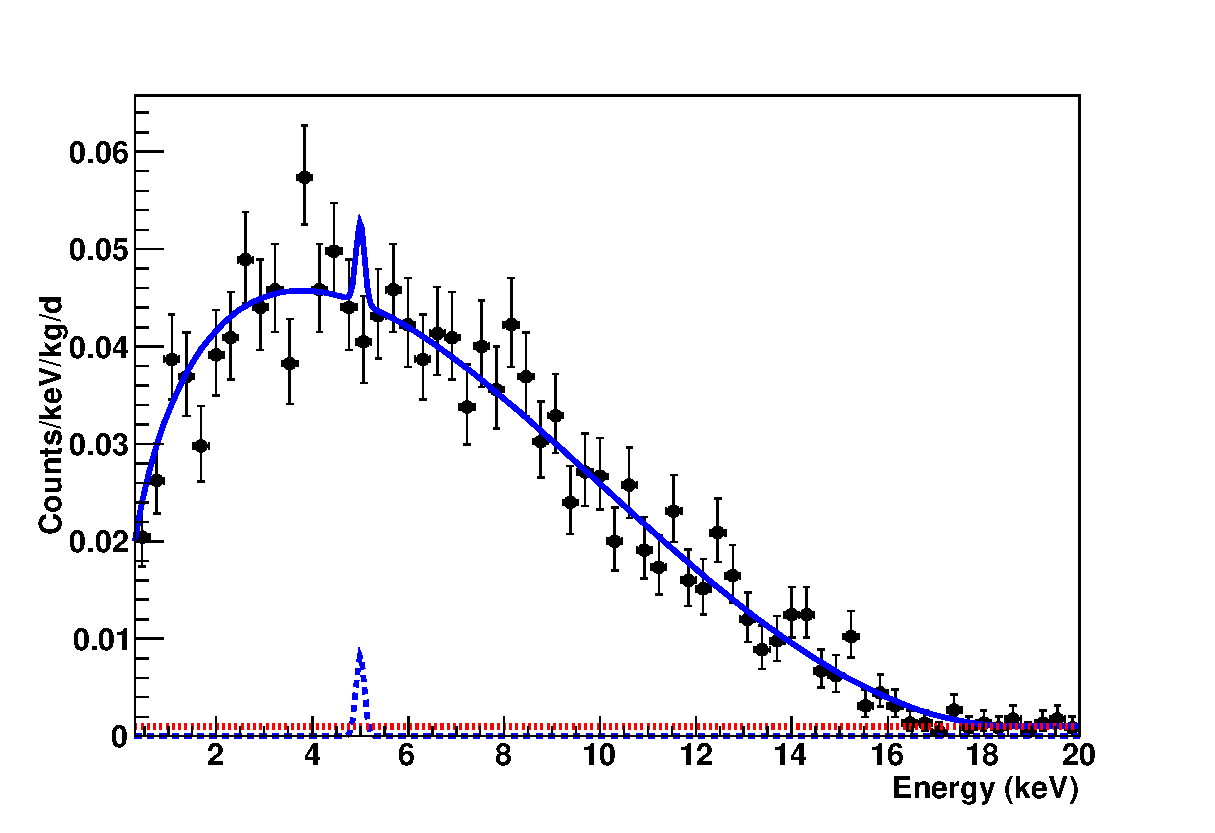
\includegraphics[width=0.9\textwidth]{MJDemoExampleSensFitAxion}
				\caption[\MJ~\minmod axioelectric sensitivity fit example.]{A sensitivity fit example 
				with axioelectric signal at $m_{a}=5$~keV, with $\gaa$ excluded at 90\% CL with
				value
				 $2.4\times10^{-11}$~pb.  Components of the fit are broken out including WIMP 
				 signal (blue dashed) and flat background (red dotted).  The major feature in the 
				 fit is due to the beta spectrum of tritium.}
				\label{fig:MJSensitivityToAxionExample}
			\end{figure}
	
			\begin{figure}
				\centering
				\def\figheight{0.41\textheight}
				\subfigure[1~year (20 kg-yr) exposure time]{
					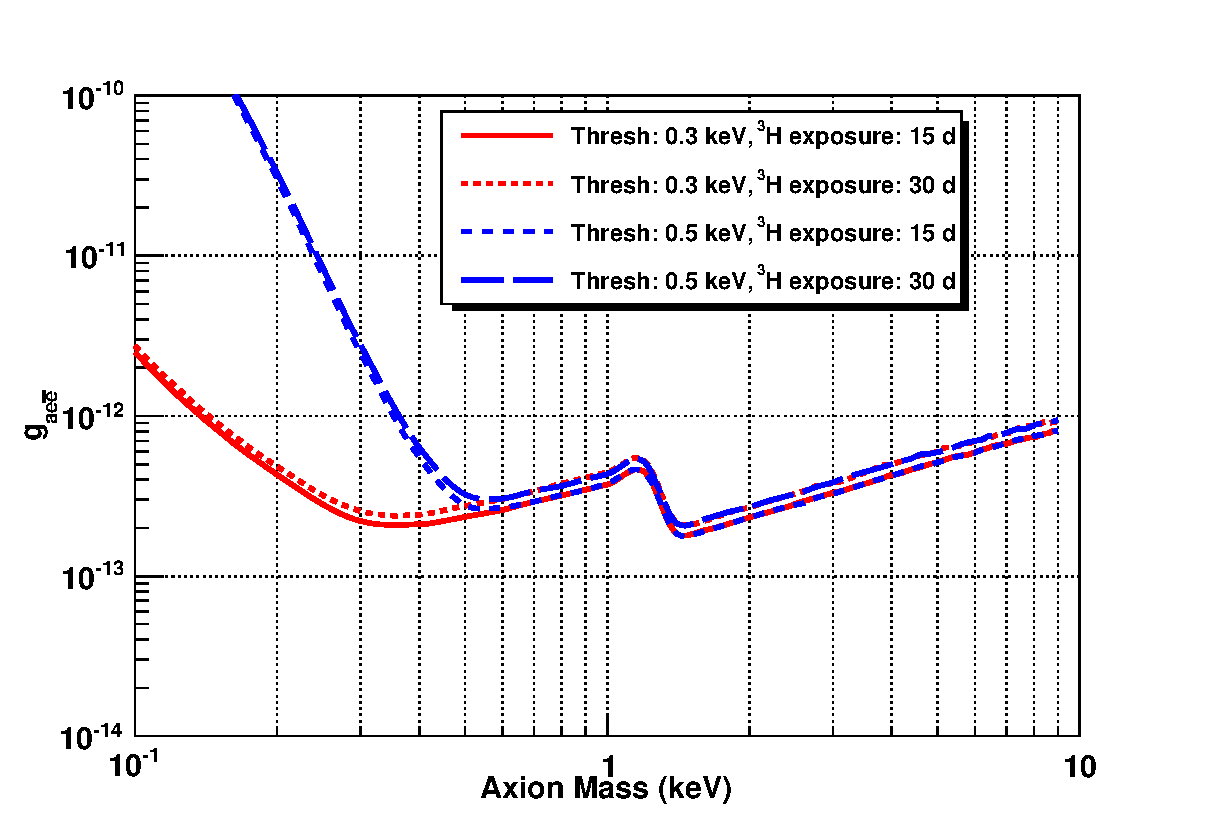
\includegraphics[height=\figheight]{1TimeExposureMJAxion}
					\label{fig:20TimeExposureMJAxion}						
				}
				\subfigure[5~year (100 kg-yr) exposure time]{
					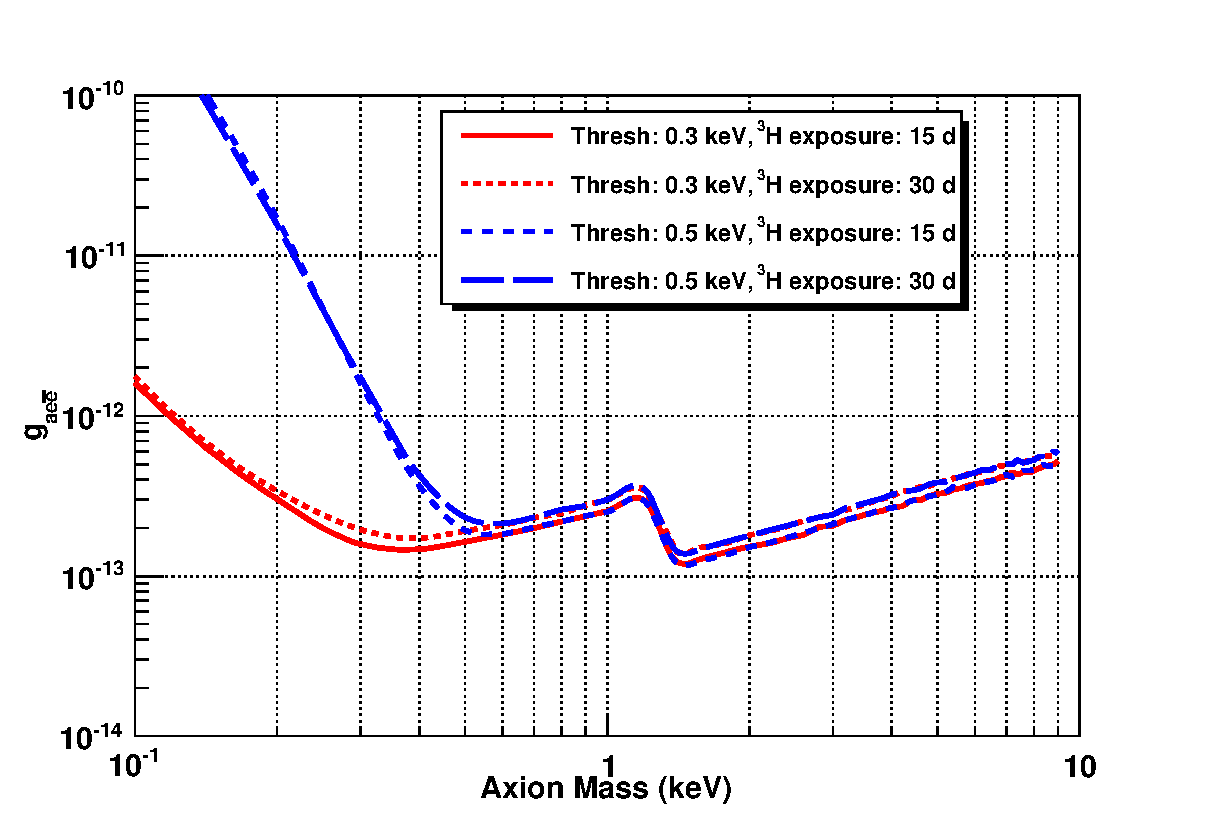
\includegraphics[height=\figheight]{5TimeExposureMJAxion}
					\label{fig:100TimeExposureMJAxion}						
				}				
				\caption[\MJ~\minmod~sensitivity to an axioelectric signal]{
				\MJ~\minmod~sensitivity to an axioelectric signal.}
				\label{fig:MJSensitivityToAxion}
			\end{figure}	
					
			\begin{figure}
				\centering
				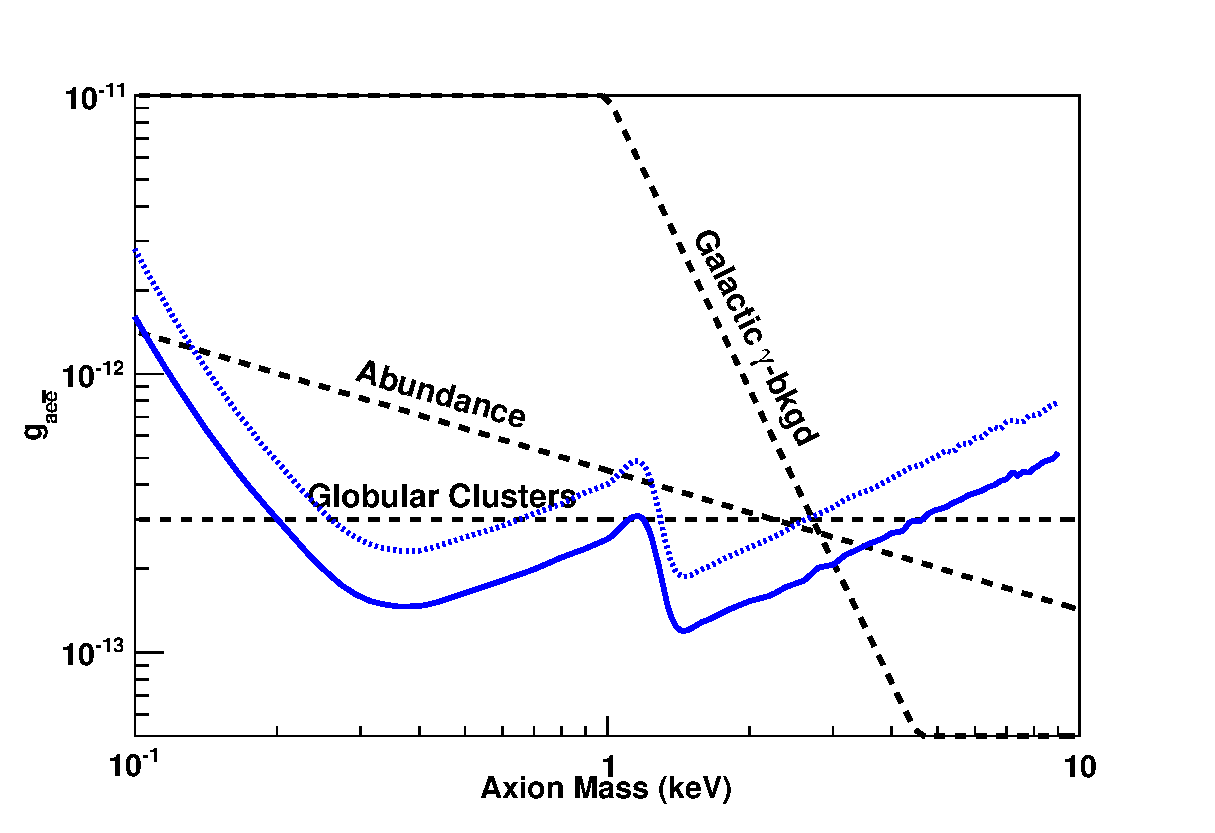
\includegraphics[width=0.9\textwidth]{MJAxionCompare}
				\caption{\MJ~\minmod~sensitivity to a Heavy Axion signal, comparing to other 
				experiments.}
				\label{fig:MJSensitivityToHeavyAxionsCompare}
			\end{figure}							

	\section{Conclusions}
	\label{sec:OtherLowEnergyConclusions}	